\chapter{Cargas, correntes e condução}\label{ch:b2:charges-currents-conduction}

Acione o interruptor e a lâmpada acende no ato; e no entanto os elétrons no
fio de cobre derivam em direção a ela a uma fração de milímetro por segundo,
e levariam horas para chegar. Um raio conduz trinta
mil ampères por um canal da largura de um dedo; o nervo
que move esse dedo conduz picoampères. O volume do Ano 1 tratou as
correntes como números em fios, $I = U/R$; este capítulo as descreve como
um \emph{campo} --- uma \omterm{def:b2:charges-currents-conduction:densities}{densidade de corrente} em cada ponto da matéria ---, escreve
a lei segundo a qual a carga nunca é criada nem destruída, e deduz a lei de Ohm
do vaivém dos elétrons num metal: o quadro microscópico
por trás do resistor, do fusível e do sensor Hall.

\begin{omfigure}
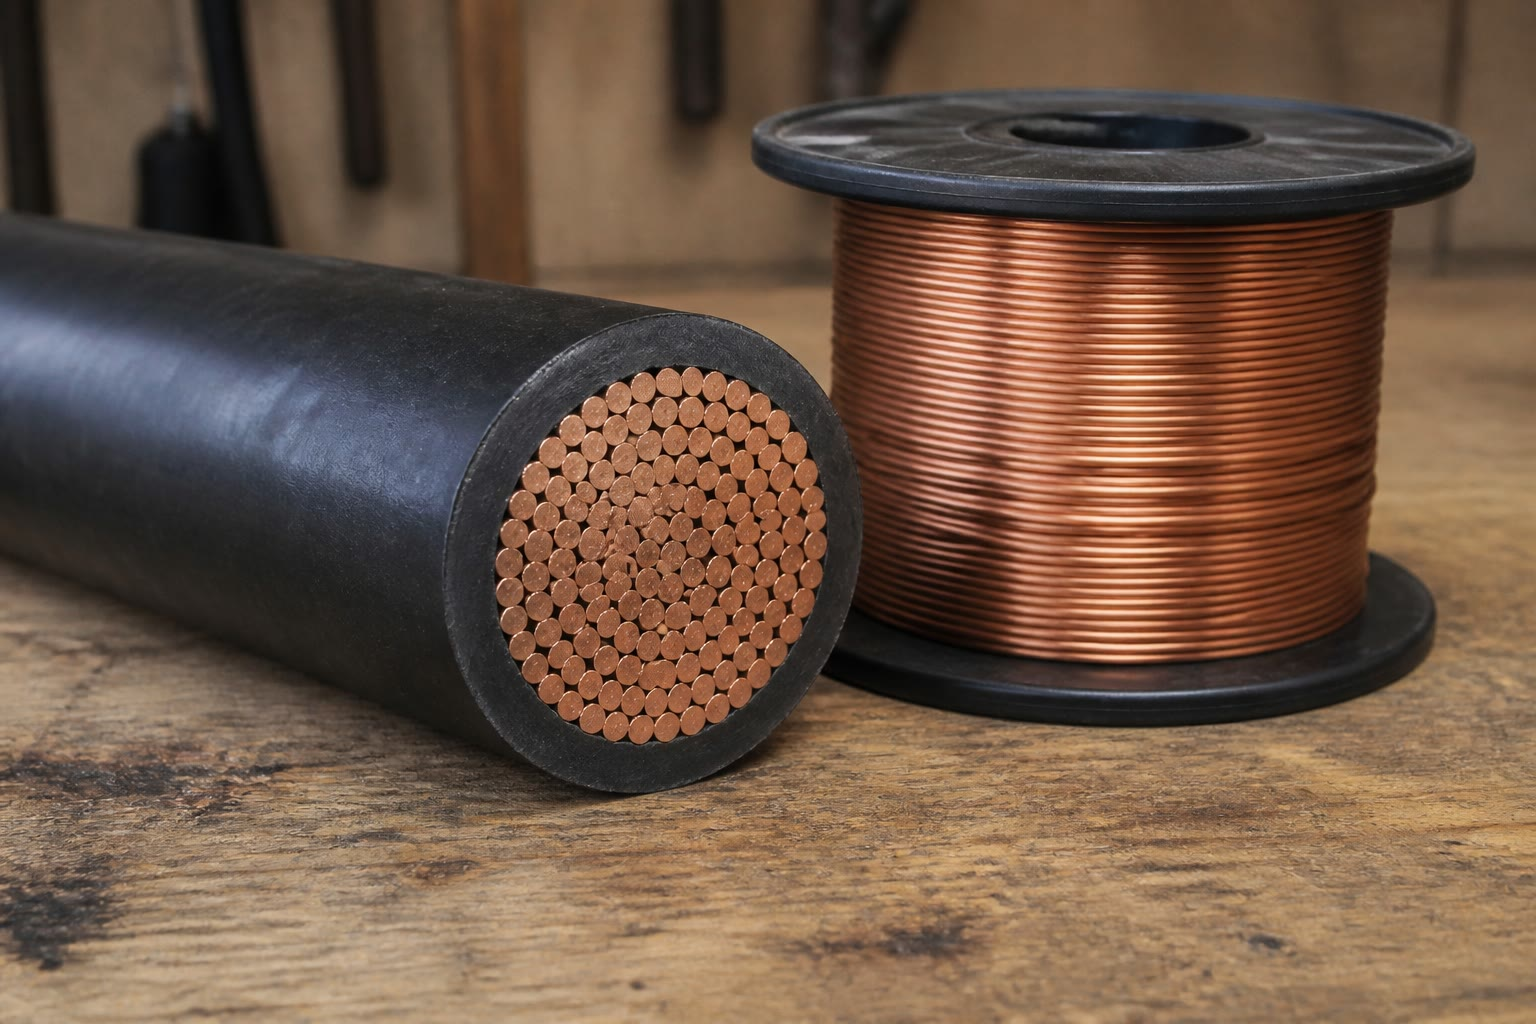
\includegraphics[width=0.58\linewidth]{images/book4/ai/b4-10-copper-wire-cable.jpg}

{\small O cobre, o condutor do mundo elétrico: nos fios deste cabo cerca de $10^{29}$ elétrons por metro cúbico derivam a uma fração de milímetro por segundo.}
\end{omfigure}


\section{Densidades de carga e de corrente}

\begin{definition}[Densidade de carga; densidade de corrente]\label{def:b2:charges-currents-conduction:densities}
\index{densidade de carga}\index{densidade de corrente}\index{intensidade (fluxo de j)}
Na \omterm{def:b2:fluid-kinematics:particle}{escala mesoscópica}, a matéria carrega uma \emph{densidade volumétrica de carga}
$\rho(M, t)$ (\unit{C/m^3}): a carga $\rho\,\dd\tau$ em $\dd\tau$. Uma superfície
pode carregar uma \emph{densidade superficial} $\sigma$ (\unit{C/m^2}), e um fio uma
densidade linear $\lambda$ (\unit{C/m}). Se os portadores da espécie $i$ (carga
$q_i$, densidade numérica $n_i$) se movem com velocidade média $\vect v_i$, a
\emph{densidade de corrente} vale
\[
\vect j = \sum_in_iq_i\,\vect v_i \qquad (\unit{A/m^2}) ,
\]
e a \emph{intensidade} através de uma superfície orientada $S$ é o fluxo
$I = \iint_S\vect j\cdot\vect n\,\dd S$: a carga que atravessa $S$ por unidade de
tempo. Para uma única espécie, $\vect j = \rho_m\vect v$ com $\rho_m = nq$ a
densidade de carga móvel.
\end{definition}

\begin{proof}
Em $\dd t$ os portadores da espécie $i$ que atravessam $\dd S$ são os que estão no
cilindro oblíquo de base $\dd S$ e geratriz $\vect v_i\dd t$: em número
$n_i\vect v_i\cdot\vect n\,\dd S\,\dd t$, com carga $q_i$ vezes isso.
\end{proof}

\begin{example}[Como os elétrons derivam devagar]\label{ex:b2:charges-currents-conduction:drift}
\index{velocidade de deriva}
O cobre tem um elétron de condução por átomo: $n = \rho_{\text{Cu}}N_A/M =
8900 \times 6.02 \times 10^{23}/0.0635 = \qty{8.5e28}{m^{-3}}$. Uma corrente de
\qty{10}{A} num fio de \qty{1.5}{mm^2} dá $j = \qty{6.7e6}{A/m^2}$, e a
\emph{\omterm{ex:b2:charges-currents-conduction:drift}{velocidade de deriva}} vale $v = j/ne = 6.7 \times 10^6/(8.5 \times 10^{28} \times 1.6 \times
10^{-19}) = \qty{0.5}{mm/s}$ --- duas horas por metro. A lâmpada acende no
ato porque o \emph{campo} que empurra os elétrons se estabelece
ao longo de todo o fio em nanossegundos (ele viaja quase à
velocidade da luz, como mostrou o cabo do \cref{ch:b2:dispersion-wave-packets}):
todos os elétrons partem juntos, como a água numa mangueira cheia.
\end{example}

\begin{omfigure}
\begin{tikzpicture}[font=\small, x=1cm, y=1cm, >=Stealth]
  \begin{scope}
    \draw[thick, omDef] (-2.6,0.7) .. controls (-1,0.9) and (0.5,0.3) .. (2.6,0.5);
    \draw[thick, omDef] (-2.6,-0.7) .. controls (-1,-0.9) and (0.5,-0.3) .. (2.6,-0.5);
    \draw[thick, omDef] (-2.6,0) ellipse (0.2 and 0.7); \draw[thick, omDef] (2.6,0) ellipse (0.15 and 0.5);
    \foreach \y in {-0.4,0,0.4} \draw[omThm, thick, ->] (-1.6,{\y*1.1}) -- (-0.6,{\y*0.9});
    \foreach \y in {-0.3,0,0.3} \draw[omThm, thick, ->] (0.8,{\y*0.9}) -- (1.9,{\y*0.8});
    \node[omThm, font=\footnotesize] at (-1.1,1.25) {$\vect j$};
    \node[font=\footnotesize] at (0,-1.4) {tubo de corrente: $I = \iint\vect j\cdot\vect n\,\dd S$ o mesmo em toda seção};
  \end{scope}
  \begin{scope}[xshift=8.0cm]
    \draw[thick, fill=omDef!10] (-2.2,-0.8) rectangle (2.2,0.8);
    \foreach \x/\y in {-1.6/0.4,-0.9/-0.3,-0.2/0.5,0.5/-0.5,1.2/0.3,1.7/-0.2} \fill (\x,\y) circle (1.4pt);
    \draw[omThm, ->] (-1.6,0.4) -- (-1.2,0.1) -- (-1.35,-0.35) -- (-0.8,-0.2) -- (-0.5,0.25);
    \draw[omDef, very thick, ->] (-0.3,-1.15) -- (1.2,-1.15) node[right, font=\footnotesize] {$\vect v$ (deriva)};
    \draw[omProp, very thick, ->] (1.2,1.15) -- (-0.3,1.15) node[left, font=\footnotesize] {$\vect E$};
    \node[font=\footnotesize] at (0,-1.6) {};
  \end{scope}
\end{tikzpicture}

{\small À esquerda: um tubo de corrente --- em regime estacionário a mesma
intensidade atravessa toda seção. À direita: um elétron num metal
ziguezagueia entre colisões a cerca de $10^6$ m/s; o campo acrescenta uma lenta
deriva, oposta a $\vect E$, de uma fração de milímetro por segundo.}
\end{omfigure}

\begin{example}[Ordens de grandeza]\label{ex:b2:charges-currents-conduction:orders}
Um raio, \qty{30}{kA} num canal de \qty{1}{cm} de raio: $j \approx \qty{1e8}{A/m^2}$.
Um fio doméstico: $10^6$--$10^7$. Um feixe de elétrons num tubo de raios catódicos,
\qty{1}{mA} em \qty{1}{mm^2}: $10^3$. Uma fibra nervosa, \qty{1}{nA} em
\qty{10}{\micro m^2}: $10^2$. O feixe de um acelerador de partículas, \qty{1}{A} numa
mancha de \qty{0.1}{mm^2}: $10^7$ --- no vácuo, sem colisão alguma.
\end{example}

\section{Conservação da carga}

\begin{theorem}[Conservação local da carga]\label{thm:b2:charges-currents-conduction:conservation}
\index{conservação da carga (local)}\index{equação da continuidade (carga)}
Em cada ponto,
\[
\frac{\partial\rho}{\partial t} + \operatorname{div}\vect j = 0 ;
\]
integrada num volume fixo $V$ limitado pela superfície fechada $\Sigma$,
$\dd Q_V/\dd t = -I_{\text{sai}}$: a carga interna só varia pelo que
atravessa a fronteira. Num \emph{regime estacionário} ($\partial_t\rho = 0$),
$\operatorname{div}\vect j = 0$: o fluxo de $\vect j$ se conserva ao longo de um tubo
de corrente, a mesma intensidade atravessa toda seção de um fio e
as correntes que entram num nó igualam as que saem (lei dos nós de Kirchhoff).
\end{theorem}

\begin{proof}
Palavra por palavra o balanço de massa de \cref{thm:b2:fluid-kinematics:continuity},
com $\rho$ a \omterm{def:b2:charges-currents-conduction:densities}{densidade de carga} e $\vect j$ sua corrente: a saída líquida
de carga pelas seis faces de uma caixa fixa, por unidade de volume, vale
$\operatorname{div}\vect j$, e nenhuma carga é criada. A forma integral soma
as caixas (as faces interiores se cancelam). Para um tubo entre duas seções
$S_1$, $S_2$ sem fluxo lateral, $I_1 = I_2$; um nó é um
volume pequeno com vários fios: $\sum I_{\text{ent}} = \sum I_{\text{sai}}$.
\end{proof}

\begin{remark}[Onde a corrente para: o capacitor]\label{rem:b2:charges-currents-conduction:capacitor}
Um fio que alimenta a placa de um capacitor é um tubo de corrente que termina: o
fluxo de $\vect j$ para dentro da placa vale $I = \dd Q/\dd t$, e carga se acumula
--- $\operatorname{div}\vect j \ne 0$ ali, e o regime não é estacionário.
E, no entanto, a mesma corrente $I$ circula no fio do outro lado: algo
deve levar o balanço através do vão. O \cref{ch:b2:maxwell-equations}
lhe dá nome --- a corrente de deslocamento --- e faz da conservação da
carga a pedra angular das equações de Maxwell.
\end{remark}

\section{O modelo de Drude e a lei de Ohm}

\begin{proposition}[Modelo de Drude; lei de Ohm local]\label{prop:b2:charges-currents-conduction:drude}
\index{modelo de Drude}\index{lei de Ohm (local)}\index{condutividade}\index{resistividade}\index{mobilidade}
Modele os elétrons de condução de um metal como partículas livres (massa $m$,
carga $-e$, densidade $n$) que sentem o campo $\vect E$ e, em média,
perdem sua quantidade de movimento de deriva por colisões com a rede a cada $\tau$
segundos --- uma \omterm{def:b2:rigid-body-mechanics:contact}{força de atrito} $-m\vect v/\tau$ sobre a velocidade média:
\[
m\frac{\dd\vect v}{\dd t} = -e\vect E - \frac m\tau\vect v .
\]
Num campo constante a deriva se estabelece, em alguns $\tau$, em $\vect v = -e\tau
\vect E/m$, e a \omterm{def:b2:charges-currents-conduction:densities}{densidade de corrente} vale
\[
\vect j = \gamma\,\vect E , \qquad \gamma = \frac{ne^2\tau}{m} :
\]
a \emph{lei de Ohm local}, com $\gamma$ a \emph{condutividade}
(\unit{S/m}; seu inverso $\rho_e = 1/\gamma$ é a \emph{resistividade},
\unit{\ohm.m}). A razão $\mu = e\tau/m$ entre a celeridade de deriva e o campo é a
\emph{mobilidade} (\unit{m^2/(V.s)}). Para um condutor de comprimento $L$ e
seção uniforme $S$ percorrido por um $\vect j$ uniforme, integrar $E = j/\gamma$
ao longo do comprimento dá $U = EL = (L/\gamma S)I$: a resistência $R = L/\gamma S
= \rho_eL/S$ do volume do Ano 1.
\end{proposition}

\begin{proof}
Com $\vect v = -e\tau\vect E/m$, $\vect j = -ne\vect v = (ne^2\tau/m)\vect E$. O
transitório $\vect v(t) = \vect v_\infty(1 - \eu^{-t/\tau})$ dura $\tau \sim
\qty{1e-14}{s}$, instantâneo em qualquer escala de tempo de circuito. A resistência
segue de $\int\vect E\cdot\dd\vect l$ entre as extremidades.
\end{proof}

\begin{example}[O cobre, a partir da condutividade medida]\label{ex:b2:charges-currents-conduction:copper}
Cobre: $\gamma = \qty{6.0e7}{S/m}$, $n = \qty{8.5e28}{m^{-3}}$: $\tau = m\gamma/ne^2 =
9.1 \times 10^{-31} \times 6 \times 10^7/(8.5 \times 10^{28} \times 2.56 \times 10^{-38}) = \qty{2.5e-14}{s}$
--- vinte e cinco femtossegundos entre colisões. A celeridade aleatória dos
elétrons num metal é de cerca de \qty{1.6e6}{m/s} (um efeito quântico, e não a
térmica $\sqrt{3k_BT/m} \approx \qty{1e5}{m/s}$), de modo que o livre caminho médio vale $\ell
= v\tau \approx \qty{40}{nm}$, cem espaçamentos atômicos: os elétrons não
colidem com os próprios átomos (um cristal perfeito é transparente para
eles), mas com seus defeitos e com as vibrações térmicas --- e é por isso que
$\gamma$ cai quando um metal é aquecido ou ligado. Mobilidade $e\tau/m =
\qty{4.4e-3}{m^2/(V.s)}$: \qty{4}{mm/s} por volt por metro.
\end{example}

\begin{proposition}[A lei de Ohm em alta frequência]\label{prop:b2:charges-currents-conduction:acdrude}
\index{condutividade complexa}
Para um campo senoidal $\underline{\vect E}\,\eu^{\iu\omega t}$ a equação de Drude
dá $\underline{\vect j} = \underline\gamma(\omega)\underline{\vect E}$ com
\[
\underline\gamma(\omega) = \frac{\gamma_0}{1 + \iu\omega\tau} , \qquad \gamma_0 = \frac{ne^2\tau}{m} :
\]
a condutividade é real e igual a seu valor em contínua enquanto $\omega\tau
\ll 1$, ou seja, até cerca de \qty{1e13}{Hz} no cobre --- por toda a faixa
de rádio e de micro-ondas; no infravermelho e no visível ($\omega\tau \gg 1$)
ela se torna imaginária, $\underline\gamma \approx ne^2/\iu m\omega$: os elétrons
oscilam livremente, fora de fase com o campo, e o metal se comporta
como o plasma do \cref{ch:b2:waves-in-media}.
\end{proposition}

\begin{proof}
$\iu\omega m\underline{\vect v} = -e\underline{\vect E} - m\underline{\vect v}/\tau$, donde
$\underline{\vect v} = -e\tau\underline{\vect E}/m(1 + \iu\omega\tau)$ e $\underline{\vect j}
= -ne\underline{\vect v}$.
\end{proof}

\begin{omfigure}
\begin{tikzpicture}
\begin{axis}[omaxis, axis x line=bottom, axis y line=left, width=7.6cm, height=4.6cm,
    xmode=log, xmin=0.01, xmax=100, ymin=0, ymax=1.1, xlabel={$\omega\tau$}, ylabel={$\underline\gamma/\gamma_0$},
    xtick={0.01,0.1,1,10,100}, ytick={0,0.5,1}, samples=200,
    xlabel style={at={(axis description cs:0.5,-0.2)}, anchor=north},
    ylabel style={at={(axis description cs:-0.12,0.5)}, rotate=90, anchor=south},
    legend style={font=\scriptsize, at={(0.97,0.95)}, anchor=north east, draw=none, fill=none}]
  \addplot[omThm, thick, domain=0.01:100] {1/(1+x*x)};
  \addplot[omDef, thick, domain=0.01:100] {x/(1+x*x)};
  \legend{$\operatorname{Re}$, $-\operatorname{Im}$}
\end{axis}
\end{tikzpicture}
\hfill
\begin{tikzpicture}[font=\small, x=1cm, y=1cm, >=Stealth]
  \draw[thick, fill=omExo!15] (-2.2,-0.6) rectangle (2.2,0.6);
  \draw[omThm, very thick, ->] (-3.0,0) -- (-2.25,0) node[above, pos=0.3, font=\footnotesize] {$I$};
  \draw[omThm, very thick, ->] (2.25,0) -- (3.0,0);
  \foreach \x in {-1.5,-0.5,0.5,1.5} \node[omProp, font=\footnotesize] at (\x,0.0) {$\otimes$};
  \node[omProp, font=\footnotesize] at (1.5,0.95) {$\vect B$};
  \draw[omDef, thick, ->] (0,0.25) -- (0,-0.4) node[right, font=\footnotesize, pos=0.5] {$\vect E_H$};
  \fill[omDef] (-0.6,0.6) circle (1.3pt); \fill[omDef] (-0.6,-0.6) circle (1.3pt);
  \node[omDef, font=\footnotesize] at (-0.9,0.85) {$+$}; \node[omDef, font=\footnotesize] at (-0.9,-0.85) {$-$};
  \node[font=\footnotesize] at (0,-1.3) {$\vect E_H = -\dfrac1{nq}\,\vect j\wedge\vect B$};
\end{tikzpicture}

{\small À esquerda: a condutividade de Drude em função de $\omega\tau$ --- real e
constante em baixa frequência, imaginária além de $1/\tau$. À direita: o efeito
Hall numa fita condutora --- os portadores são empurrados de lado pelo
campo, carregam as bordas, e o campo Hall transversal equilibra a
força magnética.}
\end{omfigure}

\begin{remark}[Condutores, semicondutores, eletrólitos]\label{rem:b2:charges-currents-conduction:materials}
\index{semicondutor}\index{eletrólito}
A mesma lei $\vect j = \sum n_iq_i\mu_i\vect E$ vale para todo condutor;
o que muda são $n$ e $\mu$. Metais: $n \sim 10^{29}$, $\gamma \sim 10^7$
S/m. Semicondutores: $n \sim 10^{16}$--$10^{23}$, fixado pela dopagem e crescendo
acentuadamente com a temperatura, com dois tipos de portadores (elétrons e
lacunas) --- donde os termistores e os diodos. Eletrólitos: íons de ambos os
sinais, $\mu \sim 10^{-8}$--$10^{-7}$ m$^2$/(V s); água do mar $\gamma \approx \qty{5}{S/m}$,
água de torneira $10^{-2}$, água pura $10^{-5}$. Isolantes (vidro, polímeros):
$\gamma \lesssim 10^{-12}$ S/m. O efeito Hall do volume do Ano 1, na
forma local $\vect E_H = -\vect j\wedge\vect B/nq$, mede $n$ e o sinal
de $q$: no alumínio ou no zinco os portadores acabam sendo positivos ---
lacunas --- e nenhum modelo clássico explica isso.
\end{remark}

\section{Energia: a lei de Joule local}

\begin{proposition}[Lei de Joule local]\label{prop:b2:charges-currents-conduction:joule}
\index{lei de Joule (local)}
O campo elétrico entrega aos portadores, por unidade de volume e de tempo,
a potência $\vect j\cdot\vect E$; num condutor ôhmico ela vale
\[
p = \vect j\cdot\vect E = \gamma E^2 = \frac{j^2}\gamma \ \ (\unit{W/m^3}) ,
\]
tudo isso convertido em calor pelas colisões (a energia cinética de
deriva é desprezível e constante). Integrada num fio, $\int j^2/\gamma\,\dd\tau
= (L/\gamma S)I^2 = RI^2$.
\end{proposition}

\begin{proof}
A força $q\vect E$ sobre cada portador trabalha à taxa $q\vect E\cdot\vect v$;
somada sobre os $n\,\dd\tau$ portadores: $nq\vect v\cdot\vect E\,\dd\tau = \vect j\cdot
\vect E\,\dd\tau$ (a força magnética não realiza trabalho). No regime
permanente de Drude essa potência é igual à dissipada pelo termo de atrito, ou seja,
transferida à rede.
\end{proof}

\begin{example}[Um fio que aquece]\label{ex:b2:charges-currents-conduction:heating}
O fio de \qty{1.5}{mm^2} a \qty{10}{A}: $p = j^2/\gamma = (6.7 \times 10^6)^2/6 \times 10^7 =
\qty{7.4e5}{W/m^3}$, ou seja, \qty{1.1}{W} por metro --- facilmente evacuados pelo ar
em volta. Deixado por conta própria (sem resfriamento), o cobre ($c = \qty{385}{J/(kg.K)}$,
$\rho = \qty{8900}{kg/m^3}$) aqueceria a $p/\rho c = \qty{0.2}{K/s}$. A \qty{100}{A}
no mesmo fio a taxa é cem vezes maior, \qty{20}{K/s}: ele
funde em um minuto --- o princípio do fusível, cujo fio fino é
feito para fundir primeiro.
\end{example}

\begin{proposition}[Relaxação da carga num condutor]\label{prop:b2:charges-currents-conduction:relaxation}
\index{tempo de relaxação (condutor)}
Num condutor ôhmico uma densidade volumétrica de carga decai como $\rho(t) =
\rho_0\eu^{-t/\tau_r}$ com
\[
\tau_r = \frac{\varepsilon_0}{\gamma} :
\]
\qty{1.5e-19}{s} para o cobre, \qty{2e-12}{s} para a água do mar, \qty{10}{s} para o vidro.
Até frequências da ordem de $1/\tau_r$ um condutor não carrega \emph{nenhuma
carga em volume}: todo excesso de carga corre para a superfície. A palavra
"condutor" depende, portanto, da escala de tempo: a água do mar é condutora
para ondas de rádio e isolante para a luz visível.
\end{proposition}

\begin{proof}
Conservação da carga com $\vect j = \gamma\vect E$ e a lei de Gauss na forma
local, $\operatorname{div}\vect E = \rho/\varepsilon_0$ (\cref{ch:b2:maxwell-equations}):
$\partial_t\rho = -\gamma\operatorname{div}\vect E = -(\gamma/\varepsilon_0)\rho$.
\end{proof}

\begin{method}[Da lei local à lei integral]\label{met:b2:charges-currents-conduction:method}
Para achar a resistência de um condutor de forma qualquer: (1) use a
simetria para escrever $\vect j$ (em regime estacionário seu fluxo se conserva, de modo que num
tubo $j \times$ seção $= I$); (2) $\vect E = \vect j/\gamma$; (3) integre
$\vect E$ ao longo de uma linha de um eletrodo ao outro: $U = \int\vect E\cdot
\dd\vect l$, e $R = U/I$; (4) confira com a potência Joule $\int j^2/\gamma\,
\dd\tau = RI^2$. Os mesmos passos dão a fuga de um cabo, a resistência
do solo em torno de um para-raios ou a de um contato cônico.
\end{method}

\section{Exercícios}

\begin{exercise}[$\star$]\label{exo:b2:charges-currents-conduction:1}
Um fio de cobre de \qty{2.5}{mm^2} conduz \qty{16}{A}. \omterm{def:b2:charges-currents-conduction:densities}{Densidade de corrente}, celeridade
de deriva ($n = \qty{8.5e28}{m^{-3}}$), tempo que um elétron leva para percorrer os
\qty{20}{m} até uma tomada; campo elétrico no fio ($\gamma = \qty{6.0e7}{S/m}$),
queda de tensão em \qty{20}{m} e potência perdida.
\end{exercise}

\begin{exercise}[$\star$]\label{exo:b2:charges-currents-conduction:2}
\omterm{def:b2:charges-currents-conduction:densities}{Densidades de corrente}: uma descarga de raio (\qty{30}{kA}, raio \qty{1}{cm}); um
feixe de elétrons (\qty{2}{mA}, \qty{0.5}{mm^2}); um axônio nervoso (\qty{1}{nA}, raio
\qty{2}{\micro m}); a corrente em anel da magnetosfera terrestre (\qty{1}{MA} por
cerca de \qty{1e14}{m^2}). Quais superam o fio do exercício anterior?
\end{exercise}

\begin{exercise}[$\star$]\label{exo:b2:charges-currents-conduction:3}
Resistividades a \qty{20}{\degreeCelsius}: cobre \qty{1.7e-8}{\ohm.m}, alumínio
\qty{2.8e-8}{\ohm.m}, ferro \qty{1.0e-7}{\ohm.m}, níquel-cromo \qty{1.1e-6}{\ohm.m}.
Resistência de \qty{100}{m} de \qty{2.5}{mm^2} em cada um; seção de alumínio
equivalente a \qty{2.5}{mm^2} de cobre, e a razão de massas (massas específicas
$8900$ e \qty{2700}{kg/m^3}); comprimento de fio de níquel-cromo de \qty{0.5}{mm} para um
aquecedor de \qty{1}{kW} e \qty{230}{V}.
\end{exercise}

\begin{exercise}[$\star$]\label{exo:b2:charges-currents-conduction:4}
Drude: $\tau$, mobilidade e livre caminho médio (celeridade aleatória \qty{1.6e6}{m/s})
para o cobre ($\gamma = \qty{6.0e7}{S/m}$, $n = \qty{8.5e28}{m^{-3}}$) e para a prata
($\gamma = \qty{6.3e7}{S/m}$, $n = \qty{5.9e28}{m^{-3}}$); condutividade de uma
amostra de silício com $n = \qty{1e22}{m^{-3}}$ e $\mu = \qty{0.14}{m^2/(V.s)}$;
celeridade de deriva nessa amostra a \qty{1}{kV/m}.
\end{exercise}

\begin{exercise}[$\star\star$]\label{exo:b2:charges-currents-conduction:5}
Um capacitor de placas $S$ é carregado por um fio com $I(t)$. (a) Aplique
a lei integral de conservação a uma superfície fechada que envolve uma placa:
relacione $I$ e a carga $Q$ da placa. (b) Por que $\operatorname{div}\vect j \ne 0$
na placa? (c) Um eletrodo esférico de raio $a$ num meio condutor
emite uma corrente radial $I$: $\vect j(r)$; verifique $\operatorname{div}
\vect j = 0$ para $r > a$ (use $\operatorname{div}\vect j = \frac1{r^2}\partial_r(r^2j_r)$
para um campo radial). (d) Onde, então, a conservação da carga
"quebra"?
\end{exercise}

\begin{exercise}[$\star\star$]\label{exo:b2:charges-currents-conduction:6}
\emph{Fuga de um \omterm{prop:b2:dispersion-wave-packets:coax}{cabo coaxial}.} O isolante entre os condutores
(raios $a = \qty{1}{mm}$, $b = \qty{3.5}{mm}$) tem $\gamma = \qty{1e-13}{S/m}$; aplica-se
uma tensão $U$ entre eles, e uma corrente radial de fuga $I$ circula
por comprimento $L$. (a) $\vect j(r)$ e $\vect E(r)$. (b) Mostre que a
resistência de um comprimento $L$ vale $R = \ln(b/a)/2\pi\gamma L$; valor por
quilômetro. (c) Corrente de fuga e potência por quilômetro a \qty{1}{kV}.
(d) Compare com a capacitância por comprimento $2\pi\varepsilon_0\varepsilon_r/\ln(b/a)$:
mostre que $RC = \varepsilon_0\varepsilon_r/\gamma$ e interprete com o tempo de relaxação.
\end{exercise}

\begin{exercise}[$\star\star$]\label{exo:b2:charges-currents-conduction:7}
\omterm{prop:b2:charges-currents-conduction:acdrude}{Condutividade complexa} do cobre ($\tau = \qty{2.5e-14}{s}$). (a) $\omega\tau$ a
\qty{50}{Hz}, \qty{10}{GHz} (micro-ondas), \qty{30}{THz} (infravermelho), \qty{5e14}{Hz}
(luz verde). (b) Módulo e fase de $\underline\gamma/\gamma_0$ em cada caso.
(c) Até que frequência a lei de Ohm vale com $1\%$ de precisão? (d) No visível,
escreva $\underline\gamma$ e mostre que $\underline{\vect j}$ está em quadratura com
$\underline{\vect E}$: potência Joule média?
\end{exercise}

\begin{exercise}[$\star\star$]\label{exo:b2:charges-currents-conduction:8}
Um fio-fusível de cobre de \qty{0.20}{mm} (cobre: $\gamma = \qty{6.0e7}{S/m}$, $\rho =
\qty{8900}{kg/m^3}$, $c = \qty{385}{J/(kg.K)}$, funde a \qty{1085}{\degreeCelsius},
calor latente \qty{205}{kJ/kg}). (a) \omterm{def:b2:charges-currents-conduction:densities}{Densidade de corrente} e potência Joule por
unidade de volume a \qty{10}{A}. (b) Tempo para fundir a partir de \qty{20}{\degreeCelsius} se nenhum
calor escapar (ignore o aumento da resistividade com a temperatura). (c)
O mesmo a \qty{30}{A}. (d) Na realidade o fio perde calor para o ar: como
isso fixa a corrente nominal de um fusível, e por que os fusíveis são selados num
cartucho cheio de areia?
\end{exercise}

\begin{exercise}[$\star\star$]\label{exo:b2:charges-currents-conduction:9}
\emph{Relaxação.} (a) Deduza $\partial_t\rho = -(\gamma/\varepsilon_0)\rho$ da conservação
da carga, da lei de Ohm e de $\operatorname{div}\vect E = \rho/\varepsilon_0$. (b)
$\tau_r$ para o cobre, a água do mar ($\gamma = \qty{5}{S/m}$), a água de torneira
(\qty{5e-2}{S/m}), o vidro (\qty{1e-12}{S/m}) e o PTFE (\qty{1e-16}{S/m}). (c)
Até que frequência cada um é um "bom condutor" (com a carga relaxando dentro de
um período)? (d) Um bastão de vidro eletrizado guarda sua carga por minutos: isso é
coerente?
\end{exercise}

\begin{exercise}[$\star\star\star$]\label{exo:b2:charges-currents-conduction:10}
\emph{Aterramento.} Um eletrodo hemisférico de raio $a = \qty{0.50}{m}$
é enterrado rente à superfície de um solo de condutividade $\gamma =
\qty{0.010}{S/m}$; uma corrente $I$ entra nele e se espalha radialmente pelo
semiespaço. (a) $\vect j(r)$, $\vect E(r)$ e o potencial $V(r)$ com $V(\infty) = 0$.
(b) Resistência do aterramento, $R = 1/2\pi\gamma a$; valor. (c) Uma
descarga de \qty{20}{kA} atinge a haste: potencial da haste;
potencial em $r = \qty{10}{m}$ e \qty{10.7}{m}; a "tensão de passo" entre
os pés de uma pessoa ali parada (pés a \qty{0.7}{m} um do outro, radialmente).
(d) Por que o gado, com as quatro patas bem afastadas, morre com
descargas próximas mais frequentemente que as pessoas?
\end{exercise}

\begin{exercise}[$\star\star\star$]\label{exo:b2:charges-currents-conduction:11}
\emph{Sensor Hall.} Uma fita de espessura $t$ e largura $w$ conduz $I$
ao longo de $x$ num campo $B$ segundo $z$. (a) A partir de $\vect E_H = -\vect j\wedge\vect B
/nq$, mostre que a tensão Hall na largura vale $V_H = IB/nqt$. (b)
Fita de cobre, $t = \qty{0.10}{mm}$, \qty{1}{A}, \qty{1}{T}: $V_H$. (c) Um
semicondutor dopado com $n = \qty{1e22}{m^{-3}}$, mesma geometria: $V_H$; por que
os sensores usam semicondutores. (d) Um sensor com $n = \qty{1e22}{m^{-3}}$, $t =
\qty{20}{\micro m}$, alimentado com \qty{1}{mA}, lê \qty{10}{\micro V}: campo medido.
O que o sinal de $V_H$ informa?
\end{exercise}

\begin{exercise}[$\star\star\star$]\label{exo:b2:charges-currents-conduction:12}
\emph{Eletrólito.} Na água, os íons Na$^+$ e Cl$^-$ têm mobilidades
$\mu_+ = \qty{5.2e-8}{m^2/(V.s)}$ e $\mu_- = \qty{7.9e-8}{m^2/(V.s)}$. (a)
Mostre que $\gamma = ne(\mu_+ + \mu_-)$ para $n$ pares de íons por unidade de volume.
(b) Água do mar, \qty{0.5}{mol/L} de NaCl: $\gamma$; compare com os \qty{5}{S/m}
medidos. (c) Celeridades de deriva a \qty{10}{V/m}; que íon carrega mais
corrente? (d) Uma coluna de água do mar de \qty{1}{cm^2} por \qty{10}{cm} conduz
\qty{1}{A}: tensão, potência e tempo para aquecê-la em \qty{10}{K} ($c =
\qty{4.0}{kJ/(kg.K)}$); por que os géis de eletroforese são resfriados.
\end{exercise}

\section{Problema: O fio de cobre, do átomo à rede elétrica}

\begin{problem}[{Problema de fim de semana --- um metro de fio doméstico examinado
em quatro escalas: o elétron, as leis locais, o circuito e a
linha de transmissão}]
\label{pb:b2:charges-currents-conduction:1}

Cobre: massa molar \qty{63.5}{g/mol}, massa específica \qty{8900}{kg/m^3}, um
elétron de condução por átomo, condutividade $\gamma = \qty{6.0e7}{S/m}$ a
\qty{20}{\degreeCelsius}, resistividade crescente $\rho_e(T) = \rho_e(20)[1 +
\alpha(T - 20)]$ com $\alpha = \qty{4.0e-3}{K^{-1}}$; $c = \qty{385}{J/(kg.K)}$. Fio:
seção $S = \qty{2.5}{mm^2}$, comprimento \qty{1}{m}, corrente \qty{16}{A}.

\medskip
\noindent\textbf{Parte I --- Os elétrons.}
\begin{enumerate}
  \item Densidade numérica $n$ dos elétrons de condução.
  \item \omterm{def:b2:charges-currents-conduction:densities}{Densidade de corrente} e \omterm{ex:b2:charges-currents-conduction:drift}{velocidade de deriva}; quanto tempo um elétron leva
        para atravessar o metro.
  \item O $\tau$ de Drude e a mobilidade; livre caminho médio com uma celeridade
        aleatória de \qty{1.6e6}{m/s}; a quantos espaçamentos atômicos (\qty{0.26}{nm})
        isso corresponde, e o que isso diz sobre aquilo com que os elétrons
        colidem?
  \item As vibrações térmicas crescem com $T$, de modo que $\tau \propto 1/T$ grosseiramente:
        confira contra $\alpha$ perto da temperatura ambiente ($\dd\rho_e/\rho_e =
        \dd T/T$ daria $\alpha = 1/293$).
  \item Campo elétrico no fio; tensão total ao longo do metro; a
        energia cinética de deriva por elétron comparada com $k_BT$ ---
        o gás de elétrons é perturbado pela corrente?
  \item Número de elétrons que atravessam uma seção do fio por segundo.
  \item Carga dos elétrons de condução no metro de fio; a
        força que o campo exerce sobre todos eles juntos; compare com
        o peso do fio. Onde vai parar essa força (pense
        nas colisões)?
\end{enumerate}

\medskip
\noindent\textbf{Parte II --- As leis locais.}
\begin{enumerate}[resume]
  \item Potência Joule por unidade de volume e por metro.
  \item O fio, no ar, perde calor à taxa $h(T - T_a)$ por unidade de
        superfície com $h = \qty{10}{W/(m^2.K)}$ (convecção): elevação de
        temperatura de equilíbrio; verifique se a correção de resistividade
        importa.
  \item O mesmo fio embutido num isolamento que só deixa passar $h =
        \qty{2}{W/(m^2.K)}$: nova elevação de temperatura, com a
        correção de resistividade incluída (resolva o balanço).
  \item Deixado sem resfriamento algum, taxa de elevação de temperatura a \qty{16}{A}
        e a \qty{160}{A} (um curto-circuito); tempo para chegar ao ponto de
        fusão (\qty{1085}{\degreeCelsius}) no segundo caso; o que protege
        a instalação?
  \item A \qty{50}{Hz}, $\omega\tau = ?$ A lei de Ohm é afetada? (O efeito
        pelicular do \cref{ch:b2:waves-in-media} é outra questão.)
  \item Escreva o tempo de relaxação $\varepsilon_0/\gamma$ do cobre; o que ele
        implica para a \omterm{def:b2:charges-currents-conduction:densities}{densidade de carga} dentro do fio, e onde fica
        a carga que produz o campo $E$ dentro do fio?
\end{enumerate}

\medskip
\noindent\textbf{Parte III --- Conservação da carga no circuito.}
O fio alimenta um capacitor $C = \qty{100}{\micro F}$ através de um interruptor; a
corrente vale $I(t) = I_0\eu^{-t/\tau_c}$ com $I_0 = \qty{16}{A}$, $\tau_c = \qty{1}{ms}$.
\begin{enumerate}[resume]
  \item Carga que chega à placa; tensão final.
  \item Aplique $\dd Q/\dd t = -I_{\text{sai}}$ a uma superfície fechada em torno da
        placa: que lado carrega uma corrente de condução e que lado não?
        Que grandeza deve, portanto, variar no vão?
  \item Em $t = \qty{0.5}{ms}$, taxa de variação da carga da placa; se as
        placas têm \qty{1}{cm^2} e estão separadas por \qty{0.1}{mm} de ar, taxa de
        variação do campo entre elas.
  \item Mostre que $\varepsilon_0\,\dd E/\dd t \times$ área da placa é igual à corrente
        no fio --- a grandeza que o \cref{ch:b2:maxwell-equations}
        acrescenta à lei de Ampère.
  \item O fio é cortado e as duas pontas ficam a \qty{1}{mm} uma da outra no ar:
        que corrente circula (ar com $\gamma \approx \qty{1e-14}{S/m}$)? Com que
        campo o ar rompe (\qty{3}{MV/m}): que tensão no
        vão produz uma faísca?
\end{enumerate}

\medskip
\noindent\textbf{Parte IV --- A linha.}
Uma linha de \qty{230}{V} em cobre de \qty{10}{mm^2}, com \qty{500}{m} de extensão (ida e volta:
\qty{1}{km} de fio), alimenta uma fazenda que consome \qty{40}{A}.
\begin{enumerate}[resume]
  \item Resistência, queda de tensão e potência perdida na linha; fração
        da potência entregue.
  \item A mesma potência a \qty{20}{kV} com um transformador em cada ponta:
        corrente, queda e perda; conclua por que a transmissão é feita em
        alta tensão.
  \item O alumínio ($\gamma = \qty{3.6e7}{S/m}$, \qty{2700}{kg/m^3}) é usado nas
        torres: seção para a mesma resistência de \qty{10}{mm^2} de
        cobre; massa por quilômetro para os dois; por que o alumínio ganha lá
        em cima e o cobre dentro da parede.
  \item Um sensor Hall preso em torno da linha lê seu campo: para
        um alicate amperímetro com $n = \qty{1e22}{m^{-3}}$, $t = \qty{0.1}{mm}$, alimentado com
        \qty{5}{mA} num campo de \qty{0.1}{T} concentrado por um núcleo de ferro,
        a tensão Hall.
  \item Depois da carga de um dia quente o fio fica a \qty{80}{\degreeCelsius}:
        sua resistência então, e a perda adicional.
  \item Um raio atinge a linha: \qty{20}{kA} durante \qty{100}{\micro s}. Energia
        dissipada no \qty{1}{km} de fio; elevação de temperatura se nada
        escapar; \omterm{def:b2:charges-currents-conduction:densities}{densidade de corrente} --- compare com a Parte I.
  \item Faça o balanço: as cinco grandezas ($n$, $\tau$, $\gamma$, $j$, $E$) que
        descrevem o fio em cada escala, e a lei que liga cada
        par.
\end{enumerate}
\end{problem}
